\documentclass[a4paper, 12pt]{report}
\usepackage[T2A]{fontenc}
\usepackage[english, russian]{babel}
\usepackage{graphicx}
\graphicspath{{./images/}}
\usepackage[utf8]{inputenc}
\usepackage[backend=biber,bibencoding=utf8,sorting=nty,maxcitenames=2,style=numeric-comp]{biblatex}
\addbibresource{bibliography.bib}

\usepackage{color} %% это для отображения цвета в коде
\usepackage{listings} %% собственно, это и есть пакет listings
\usepackage{caption}
\DeclareCaptionFont{white}{\color{white}} %% это сделает текст заголовка белым
%% код ниже нарисует серую рамочку вокруг заголовка кода.
\DeclareCaptionFormat{listing}{\colorbox{gray}{\parbox{\textwidth}{#1#2#3}}}
\captionsetup[lstlisting]{format=listing,labelfont=white,textfont=white}

\begin{document}
	
	
	\lstset{ %
		language=C,                 % выбор языка для подсветки (здесь это С)
		basicstyle=\small\sffamily, % размер и начертание шрифта для подсветки кода
		numbers=left,               % где поставить нумерацию строк (слева\справа)
		numberstyle=\tiny,           % размер шрифта для номеров строк
		stepnumber=1,                   % размер шага между двумя номерами строк
		numbersep=5pt,                % как далеко отстоят номера строк от подсвечиваемого кода
		backgroundcolor=\color{white}, % цвет фона подсветки - используем \usepackage{color}
		showspaces=false,            % показывать или нет пробелы специальными отступами
		showstringspaces=false,      % показывать или нет пробелы в строках
		showtabs=false,             % показывать или нет табуляцию в строках
		frame=single,              % рисовать рамку вокруг кода
		tabsize=2,                 % размер табуляции по умолчанию равен 2 пробелам
		captionpos=t,              % позиция заголовка вверху [t] или внизу [b] 
		breaklines=true,           % автоматически переносить строки (да\нет)
		breakatwhitespace=false, % переносить строки только если есть пробел
		escapeinside={\%*}{*)}   % если нужно добавить комментарии в коде
	}
	
	\chapter{Защита информации в операционных системах}
	\section{Сетевое программирование на C#}
	
	 \begin{figure}[h]
		
		\centering
		
\includegraphics[width=0.5\linewidth]{full_dbGCToKq.jpg}
		
	\end{figure}

	Сегодня миллионы компьютеров и устройств связаны в глобальную сеть интернет, либо в отдельные локальные подсети. В связи с этим возникает необходимость создания приложений, которые бы использовали все преимущества передачи данных по сети. Например, одним из распространенных приложений, которое использует передачу по сети, является веб-браузер. И платформа .NET и язык программирования C# предоставляют все необходимые возможности для создания приложений, которые могут взаимодействовать по сети и использовать различные сетевые протоколы.
	
	Но прежде чем переходить непосредственно к созданию приложений, надо пару слов сказать, что вообще представляет собой коммуникация в сети.
	
	Вся сеть состоит из отдельных элементов - хостов, которые представляют собой компьютеры и другие подключенные устройства. Между собой они соединены каналами связи (кабели Ethernet, Wi-Fi и т.д.) и маршрутизаторами. Маршрутизаторы объединяют компьютеры в подсети и контролируют передачу данных между ними.
	
	Но компьютеры-хосты не взаимодействуют абы как между собой. Они применяют протоколы. Протокол представляет собой соглашения о том, как пакеты данных будут передаваться по каналам коммуникации. Таким образом, протокол упорядочивает взаимодействие.
	
	Существует множество различных протоколов. Протоколы, которые используются для передачи данных по сети, составляют семейство протоколов TCP/IP. Основные из них: Internet Protocol (IP), Transmission Control Protocol (TCP) и User Datagram Protocol (UDP). Причем эти протоколы организованы в уровневую систему (\ref{formula2})
	
	\begin{equation}
		TCPI = (BAC – EV)/(BAC – AC)
		\label{formula2}
	\end{equation}
	
	
	IP представляет сетевой уровень. Он использует нижележащие уровни, которые представляют физические каналы коммуникации - кабели Ethernet и т.д., для передачи пакетов с данными другому хосту. \cite{фунтов2021основы}
	
	Выше IP располагается транспортный уровень, который образуют протоколы TCP и UDP. Эти протоколы используют определенные порты для передачи данных. TCP позволяет отследить потерю пакетов и их дублирование при передаче. UDP подобного не позволяет сделать и нацелен на простую передачу данных.
	
	Однако приложение взаимодействует с уровнем TCP / UDP не напрямую, а через специальный API, который предоставляют сокеты. Сокеты - это не какой-либо протокол, это просто интерфейс для создания сетевых приложений, который опирается на встроенные возможности операционной системы.
	
	В зависимости от используемого протокола различают два вида сокетов: потоковые сокеты (stream socket) и дейтаграммные сокеты (datagram socket). Потоковые сокеты используют протокол TCP, дейтаграммные - протокол UDP.
	
	 \begin{figure}[h]
		
		\centering
		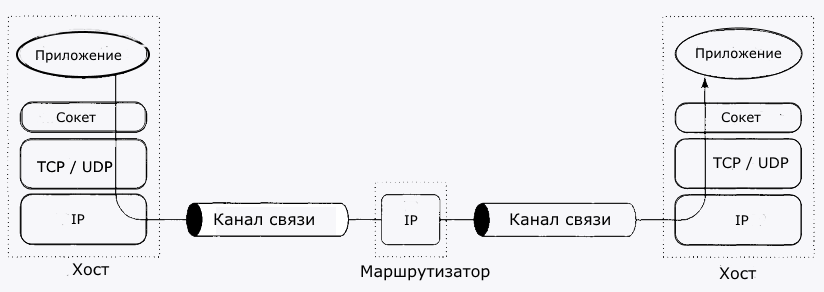
\includegraphics[width=0.5\linewidth]{protocols.png}
		
	\end{figure}
	
	В итоге, когда приложение посылает сообщение приложению, запущенному на другом хосте, то приложение обращается к сокетам для передачи данных на уровень TCP / UDP. Далее с этого транспортного уровня данные передаются сетевому уровню - уровню протокола IP. И этот протокол передает данные далее физическим уровням, и после этого данные уходят по сети.
	
	Чтобы уникально определять хосты в сети каждый хост имеет адрес. Существует несколько различных протоколов адресов. В настоящее время наиболее распространен протокол IPv4, который предполагает представление адреса в виде 32-битного числа, например, 37.120.16.63. Такой адрес содержит четыре числа, разделенных точками, и каждое число находится в диапазоне от 0 до 255. Однако также в последнее время набирает оборот использование адресов протокола IPv6, которые представляют собой 128-битное значение.
	
	\begin{figure}[h]
		
		\centering
		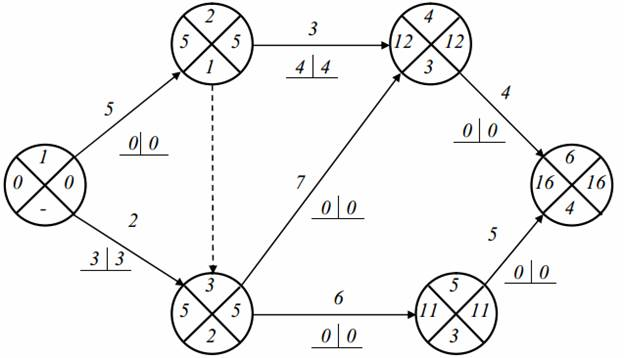
\includegraphics[width=0.5\linewidth]{image001.png}
		
	\end{figure}
	
	Однако такие адреса очень сложно запомнить, поэтому в реальности чаще оперируют доменами. Домены представляют специальные названия, используемые для интернет-адресов. Например, есть доменное имя "www.microsoft.com", ему соответствует адрес в формате IPv4 2.23.143.150. Но для протокола IP, через который идет взаимодействие, доменные адреса не существуют. Поэтому при отправке или передаче данных по доменному имени, компьютер еще обращается к службам Domain Name System (DNS), который выполняют сопоставление между интернет-адресами в формате IPv4 или IPv6 и доменными названиями.
	
	Кроме адреса при сетевых взаимодействиях используются порты. Порт представляет 16-битное число в диапазоне от 1 до 65 535. Использование портов позволяет разграничить несколько запущенных приложений на одном хосте.
	
	Ключевыми компонентами сетевого взаимодействия являются клиент и сервер. Клиент посылает запрос, а сервер получает запрос, обрабатывает его и посылает обратно клиенту некоторый ответ. Простейший пример - веб-браузер, который служит в качестве клиента, отправляя запрос на некоторый сайт. А сайт выступает в качестве сервера, отправляя браузеру некоторый ответ, который браузер затем отображает пользователю. Однако в реальности нередко одно приложение может выступать и в качестве сервера, и в качестве клиента. \cite{дубаков2013сетевое}
	
	Собственно, это все базовые принципы взаимодействия по сети, которые надо знать. В реальности, как правило, при создании приложений не потребуется глубокого знания всех протоколов и нюансов их работы. Если в редких случаях возникнет необходимость более детального знания протоколов, то в этом случае можно обратиться к специализированной литературе, в данном же руководстве мы сосредоточимся непосредственно на тех возможностях, которые предоставляет фреймворк .NET для работы с сетью.
	
	Основная функциональность фреймворка .NET по работе с сетями содержится в пакете System.Net. Также есть дополнительные пакеты:
	
	System.Net.Http: содержит функциональность по работе с протоколом HTTP
	
	System.Net.NetworkInformation: редоставляет доступ к данным о сетевом трафике и сетевых адресах, а также к прочей информации о хостах сети. Также предоставляет функциональность ping
	
	System.Net.Security: предоставляет сетевые потоки для безопасной связи между хостами
	
	System.Net.Sockets: предоставляет доступ к функциональности сокетов операционной системы
	
	System.Net.WebSockets: предоставляет доступ к реализации инфтерфейса WebSocket
	
	System.Net.Quic: содержит типы, которые реализуют протокол QUIC в соответствии со спецификацией RFC 9000.(\ref{formula})

	\begin{equation}
		R(ij)= t_p_(_j_)- t_r_(_i_)-t_i_j
		\label{formula}
	\end{equation}
	
	\chapter{Отправка и получение данных в TCP. Однонаправленная связь между сокетами}
	
	В листинге \ref{some-code} Пример сетевого программирования:
	
	\begin{lstlisting}[label=some-code,caption= Поиск основных состояний]
		using System;
		using System.Collections.Generic;
		using System.Linq;
		using System.Text;
		using System.Threading.Tasks;
		using System.Net.Sockets;
		
		namespace Krestiki_and_zeriki
		{
			class Program
			{
				static void Main(string[] args)
				{
					Socket socket = new Socket(AddressFamily.InterNetwork, SocketType.Stream, ProtocolType.Tcp);
					String a;
					Socket cl;
					byte[] mas = new byte[20];
					a = Console.ReadLine();
					if (a == "s")
					{
						socket.Bind(new System.Net.IPEndPoint(System.Net.IPAddress.Parse("127.0.0.1"), 8888));
						socket.Listen(0);
						cl = socket.Accept();
						String str = "zxzxzxzx";
						
						mas=Encoding.UTF8.GetBytes(str);
						cl.Send(mas);
					}
					else 
					{
						try
						{
							socket.Connect(new System.Net.IPEndPoint(System.Net.IPAddress.Parse("127.0.0.1"), 8888));
						}
						catch
						{
							Console.WriteLine("Сервер спит.");
							return;
						}
						int xcv = socket.Receive(mas);
						string str;
						str=Encoding.UTF8.GetString(mas,0,xcv);
						Console.WriteLine(str);
					}
				}
			}
		}
	\end{lstlisting}
	
	
	\printbibliography
	
\end{document}